\documentclass[../../main.tex]{subfiles}
\begin{document}
\section{Algorithmes et programmation}
La définition rigoureuse d'un algorithme se trouve n'être absolument pas trivial, ni même simple.
Une première raison à cela est qu'il s'agit d'un concept au départ considéré comme intuitif, et que la
formalisation d'un concept qui semble humainement intuitif pose immédiatement la question du bien
fondé et de la rigueur de cette formalisation : un mot est toujours interprété, et deux humains peuvent
utiliser le même mot, et ne pas en avoir la même utilisation, voir la même compréhension fine.

La difficulté sous-jacente à une telle définition sera tout à fait esquivé ici puisqu'elle nécessiterait
de poser une théorie du calcul pour définir ce qu'est un problème, ce que signifie la résolution d'un
problème, ainsi que la résolution en temps fini d'un problème, ce qu'est une instruction élémentaire,
etc\dots

On s'en passera en conservant une définition \og avec les mains \fg{} qui manque cruellement de rigueur
mais qui a le bénéfice d'être simple et suffisante dans un cadre purement pratique.

\definition{Algorithme}{Un algorithme est une suite d'actions/d'instructions précises dont l'objectif est de résoudre un problème donné. Ces instructions doivent être les plus élémentaires possibles, et ne surtout pas être ambigües. C'est-à-dire qu'en lisant l'algorithme, il n'y ait qu'une seule possibilité d'action à chaque étape (ce qui ne signifie pas que le résultat soit prédéterminé puisqu'une action peut potentiellement avoir un résultat aléatoire, comme le lancer d'un dé par exemple).}

\textbf{Exemple :} "Changer la valeur d'un nombre" n'est pas une instruction possible pour un algorithme, puisque le lecteur peut toujours \textit{interpréter} l'instruction, et ne sait en fait toujours pas exactement ce qu'il doit faire. Par contre l'instruction "Ajouter 1 à la valeur de la variable $x$" est une instruction, à condition que $x$ soit connue, que $1$ soit bien définie et que ``Ajouter'' soit une opération binaire bien définie sur $1$ et $x$.

Tout simplement.

\begin{algorithm}
\caption{Premier exemple simple}\label{alg:hello}
Afficher("Bonjour !")\;
Afficher("Au revoir !")\;
\end{algorithm}
Cette algorithme n'est valable que si l'opération "Afficher" a été décrite de manière super précise avant. C'est-à-dire que même l'endroit où il faut afficher (par exemple, la feuille sur laquelle est écrite ce chapitre d'algorithmique) est indiqué auparavant au lecteur, \textit{pour éviter l'interprétation}. La donnée d'une chaîne de caractère doit également être connue.

Un algorithme peut ensuite être exécuté par un \textit{agent}, et il produira alors un résultat donné.

\definition{Agent algorithmique}{Actionneur capable de communication qui lira l'algorithme écrit et effectuera les actions les unes à la suite des autres. Ce peut être un être humain, ou encore un chat ou un chien (par exemple en apprenant l'algorithme à haute voix au chien)}

L'\textbf{Algorithme 1} produira donc le résultat suivant :

\begin{minipage}{1.\textwidth} \fontfamily{pcr}\selectfont
	Bonjour !\newline
	Au revoir !
\end{minipage}

L'intérêt d'algorithmes est notamment d'automatiser des tâches. On peut notamment imaginer l'algorithme suivant :
\newline
\begin{algorithm}
\caption{Cuisson des pâtes}\label{alg:letters}
Prendre une casserole\;
Mettre de l'eau dans la casserole\;
Mettre la casserole sur le feu\;
Allumer le feu sous la casserole\;
\Tq{l'eau ne bout pas} {
	Attendre que l'eau bout\;
}
Mettre les pâtes dans la casserole\;
Attendre 9 minutes\;
\end{algorithm}

On peut imaginer apprendre cet algorithme à notre singe de compagnie (c'est pas si con les singes\dots), et simplement lui ordonner d'exécuter cet algorithme par l'instruction "Va faire cuire les pâtes !".

\textbf{Remarque :} En petit malin, le lecteur attentif peut observer\footnote{C'est la technique classique de "Nan mais t'inquiètes, tu vois l'erreur là ? C'est juste pour voir si tu suis, et pas parce-que j'ai oublié."\dots \textit{a priori} là ça va :)} que l'\textit{agent} qui exécute cet algorithme doit déjà savoir de quelle casserole, de quel feu, pâtes et eau il est question, pour qu'il n'y ait pas d'interprétation (et pour aller plus loin, il faut aussi qu'il comprenne le langage dans lequel est exprimé l'algorithme et le sens de chaque verbe/action, ce qui n'est pas toujours évident pour un singe).
\subsection{Algorithmes et programmes}
\definition{Programme}{Un programme informatique est un algorithme pouvant être exécuté par un ordinateur (qui est donc l'agent exécutant). Il doit donc être écrit dans un langage compréhensible par l'ordinateur appelé \textit{langage de programmation}.}

Dans la suite du chapitre, l'entièreté des algorithmes seront exécutés sur ordinateur, pour la principale raison que cela permet de visualiser les résultats et d'expérimenter par soi-même.

On va donc considérer pour toute la suite des programmes. Il faut cependant garder à l'esprit la distinction entre les deux, puisqu'un algorithme englobe beaucoup plus de choses qu'un programme informatique (il est difficile de programmer un ordinateur pour aller chercher le journal dans la boîte aux lettres).

Pour qu'un programme puisse être exécuté par un ordinateur, il doit être connu de celui-ci, et est donc stocké dans la mémoire de l'ordinateur. L'ordinateur va ensuite le lire instructions par instructions et exécuter chacune de ces instructions.

La représentation de l'algorithme doit donc être accessible à un ordinateur. On peut considérer une écriture de cette algorithme en langage binaire, c'est-à-dire comme une suite finie de 0 et de 1. La traduction du langage naturel (c'est-à-dire humain) en langage binaire est appellée \textit{compilation}. Elle est effectuée par des programmes appellées des \textit{compilateurs}.

On peut cependant généraliser un peu la notion de \textit{compilation} : on peut dire que compiler c'est lire une suite de caractères obéissant à une certaine syntaxe, en construisant une (autre) représentation de l'information que ces caractères expriment. De ce point
de vue, beaucoup d'opérations apparaissent comme étant de la compilation; à la limite, la lecture d'un nombre est déjà de la compilation, puisqu'il s'agit de lire des caractères constituant l'écriture d'une valeur selon la syntaxe des nombres décimaux et de fabriquer une autre représentation de la même information, à savoir sa valeur numérique \og dans notre tête \fg
\section{Un peu de vocabulaire}
Cette table de vocabulaire est donné en préambule pour ne pas trop surcharger le texte ci-après.

\definition{BIOS}{Le BIOS (\textit{\underline{B}asic \underline{I}nput \underline{O}utput \underline{S}ystem}) est le programme qui s'exécute au démarrage de l'ordinateur (appelé le \textit{boot}). C'est lui qui permet de le lancer véritablement pour être utilisé. En effet, son objectif est de ``passer la main'' au système d'exploitation, grâce à un petit programme appelé le \textit{bootloader} (\textit{loader} signifie chargeur en anglais).

\begin{minipage}{\textwidth}
	\begin{center}
		\small
		\includesvg[width=1\textwidth]{bios}
	\end{center}
\end{minipage}
}

\definition{Système d'exploitation}{Un système d'exploitation est un programme exécuté par le BIOS juste après le lancement. Ce programme fournie à l'utilisateur de l'ordinateur toutes les fonctionnalités dont il pourrait avoir besoin : accès au disque dur, accès à la mémoire vive, aux périphériques entrée/sortie, possibilité d'exécuter des programmes utilisateurs, générateur de nombres pseudo-aléatoire, etc\dots

\begin{minipage}{\textwidth}
	\begin{center}
		\includesvg[width=.7\textwidth]{niveau_abstraction}
	\end{center}
\end{minipage}
}

\definition{Fichier}{Un fichier est un ensemble d'informations numériques constituées d'une séquence d'octets. Ces informations peuvent représenter des données allant du programme informatique à la vidéo en passant par les informations d'une communication réseaux, un livre numérique, la mémoire d'un programme informatique, etc\dots Ces informations sont réunis sous un même nom et manipulé comme une unité, appelé le fichier. Les métadonnées d'un fichier fournissent des informations externes complémentaires.

\begin{minipage}{\textwidth}
	\begin{center}
		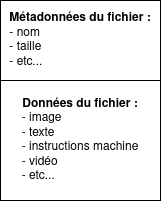
\includegraphics[width=.25\textwidth]{fichier}
	\end{center}
\end{minipage} 
}

\definition{Extension de nom fichier}{Une extension de nom de fichier (ou plus simplement ``extension de fichier'') est une suite de caractères à la fin du nom du fichier, séparée du radical du nom de fichier par un point, qui indique à l'utilisateur de l'ordinateur et aux logiciels le format des données qu'il contient. L'extension agit uniquement à titre \textit{indicatif} ! La modifier sans modifier le fichier lui-même n'effectue STRICTEMENT AUCUNE conversion. Il ne suffit pas d'appeler un chat un chien pour que celui-ci se transforme subitement ! Le nom d'un fichier est seulement une étiquette. Il n'a aucune incidence sur ce que le fichier contient réellement.\footnote{J'insiste car il s'agit là d'une \textit{croyance} extrêmement répandue chez les utilisateurs non techniciens d'outils informatiques}}

\definition{Répertoire et système de fichiers}{Un répertoire est le nom technique donné au dossier. Il s'agit simplement d'un conteneur d'autres répertoires ou fichiers. Il permet de \textit{répertorier} des fichiers ou d'autres répertoires. Sa fonction principale est donc la classification. Afin de faciliter la localisation et la gestion des répertoires et des fichiers, ceux-ci sont organisés suivant un \textit{système de fichiers}. C'est ce système qui permet à l'utilisateur de répartir les fichiers dans une arborescence de répertoires et de les localiser par un chemin d'accès.
\begin{center}
\begin{forest}
[Documents
	[repertoire\_parent
		[repertoire\_enfant\_1
			[fichier\_texte]
			[fichier\_image]
		]
		[repertoire\_enfant\_2
			[fichier\_video]
		]
	]
]
\end{forest}
\end{center}
}

\definition{Répertoire de travail}{Le répertoire de travail d'un exécutable est le répertoire dans lequel l'exécutable va effectuer ses instructions. Par exemple, si l'exécutable contient une instruction qui ouvre et lit un fichier sur le disque dur, l'ordinateur essaiera d'ouvrir ce fichier dans le répertoire de travail, renverra une erreur si ce fichier n'est pas présent dans le répertoire de travail. Il est possible de modifier le répertoire de travail d'un exécutable à l'intérieur de celui-ci (par certaines instructions).}

\definition{Chemin d'accès}{Chaîne de caractères qui décrit la position du fichier sur son support de stockage au sein du système de fichiers. On distingue deux types de chemin d'accès : 
\begin{itemize}
		 \item chemin absolu : décrit la position absolue du fichier depuis la racine de l'arborescence du système de fichiers ($/$ sous Linux, $C:/$ sous Windows)
		 \item chemin relatif : décrit la position relative du fichier par rapport au répertoire de travail. On considère alors le répertoire de travail comme la racine de l'arborescence
\end{itemize}
\begin{center}
\begin{forest}
[racine
	[...]
	[home
		[user
			[repertoire\_1]
			[
				[fichier\_1]
			]
			[repertoire\_2]
			[
				[fichier\_2]
			]
		]
	]
	[...]
]
\end{forest}
\end{center}
Ci-dessus, le chemin absolu du fichier 1 est \textit{racine/home/user/repertoire\_1/fichier\_1}. Si on suppose que le répertoire de travail est \textit{racine/home/user/repertoire\_1}, alors le chemin relatif du fichier 2 est \textit{../repertoire\_2/fichier\_2}.

En effet, ``.'' désigne le nom du répertoire de travail, et ``..'' désigne le répertoire parent du répertoire de travail. Ainsi, \textit{../repertoire\_2} désigne le chemin relatif depuis le répertoire 1 équivalent au chemin absolu \textit{racine/home/user/}
}
\definition{Instruction}{Une instruction est une séquence d'octets qui peut être lue par l'UCC pour exécuter une action.}

\definition{Exécutable}{Un fichier exécutable (ou plus simplement un exécutable) est un fichier contenant un entête d'informations générales et une séquence d'instructions. L'entête peut par exemple définir le point d'entrée du programme, c'est-à-dire l'adresse (relative) dans la séquence d'instructions à laquelle l'ordinateur doit débuter sa lecture des instructions.

\begin{minipage}{\textwidth}
	\begin{center}
		\hspace*{-3cm}\includesvg[width=.5\textwidth]{executable}
	\end{center}
\end{minipage}
}

\definition{Niveau d'abstraction}{Les langages de programmation peuvent être plus abstraits, c'est-à-dire être proche ou non du fonctionnement technique de l'ordinateur. Un langage à haut niveau d'abstraction va cacher la technique associée à la manipulation du matériel de l'ordinateur (mémoire vive, périphériques, etc\dots) tandis qu'un langage à bas niveau d'abstraction va laisser la possibilité au programmeur de manipuler lui-même ce qui est ``matériel''. En fait, les langages à haut niveau d'abstraction écrivent les instructions de manipulation bas niveau à l'insu du programmeur.

\begin{minipage}{\textwidth}
	\begin{center}
		\includesvg[width=.45\textwidth]{abstraction_langages}
	\end{center}
\end{minipage}
}
\section{Langages de programmation}
\subsection{Objectifs des langages de programmation}
Les langages dits \og de programmation \fg ont un objectif : la description de données.

Ces données peuvent être de multiples natures. Ce peut être :
\begin{itemize}
	\item un programme
	\item une page internet
	\item une base de relations entre données
	\item un fichier PDF comme celui-ci
	\item de la musique
	\item etc\dots
\end{itemize}
Il est à noter par ailleurs qu'un programme est potentiellement capable de décrire lui-même n'importe quel type information. Cependant, certains langages de programmation décrivent directement les données et non pas le programme qui les génère. On appelle les langages de programmation décrivant directement les données des \textit{langages de description}. Les langages décrivant des instructions exécutables par un ordinateur sont appellés des \textit{langages impératifs}.
\subsection{Langages compilés et interprétés}
Les langages de programmation peuvent être à nouveau divisés en deux catégories distinctes :
\begin{itemize}
	\item les langages compilés
	\item les langages interprétés
\end{itemize}
La compilation consiste à traduire un texte écrit dans un langage de programmation sous une forme accessible par un ordinateur, c'est-à-dire en langage binaire généralement.

Certains langages de programmation nécessitent d'être compilés pour que la donnée décrite puisse être traitée par l'ordinateur. Par exemple, la description en LaTex d'un document nécessite une compilation par un autre programme pour être codée au format PDF. Les langages C, C++ et Assembleur sont également des langages qui nécessitent un \textit{compilateur} pour être transformés/traduits en code binaire qui puisse être exécuté par un ordinateur.

L'autre catégorie de langages, dits interprétés, n'est jamais traduite en langage binaire pour être exécuté par l'ordinateur directement. Il y a à la place une interface créée par un autre programme appellé \textit{interpréteur}. Ce programme, qui lui est exécuté par l'ordinateur, va simuler l'exécution de l'ordinateur sur le code. Il va lire chacune des lignes du programme écrit, et va faire exécuter les instructions correspondantes à l'ordinateur. Cela permet notamment de créer un niveau d'abstraction supplémentaire pour le programmeur, qui n'a pas besoin de connaître sa machine pour écrire des programmes. C'est l'interpréteur qui s'occupe de l'aspect le plus technique. Le désavantage majeur de ce type de langages interprétés est que l'exécution d'un programme est beaucoup plus lente puisqu'une étape de traduction ``en direct'' par l'interpréteur est nécessaire \textbf{à chaque exécution du programme}. Ce type de langages n'a pu se développer efficacement que lorsque les ordinateurs ont été assez puissants pour le permettre.\footnote{\textit{Fun fact} : le langage interprété Lisp était très utilisé en intelligence artificielle au XX$^e$ siècle. Comme les ordinateurs généralistes de l'époque étaient trop lents, des ordinateurs spécialisés pour interpréter ce langages ont été développés : \href{https://fr.wikipedia.org/wiki/Machine_Lisp}{les machines Lisp}.} Cela explique par exemple l'explosion de Python dans le monde du développement ces dix dernières années.\footnote{Avis personnel de l'auteur : utiliser des langages qui consomment beaucoup plus de ressources pour arriver au même résultat avec des performances moindres pour des seules raisons de facilité est un problème dans un monde qui a besoin d'une baisse drastique de la consommation énergétique pour sa survie. Le Python ne permet pas de comprendre en profondeur les choses ni d'optimiser les programmes écrits de manière réellement efficace. Il n'est donc pas adapté pour des projets de grande envergure mais reste parfois utile pour tester une idée en cinq minutes. Certains argueront que le langage est utilisé à profusion dans le monde de l'industrie. Il s'agit pour moi d'une erreur à but lucrative mais non pérenne. À discuter\dots}
\section{Le langage C}
Le langage C est un langage de bas niveau, c'est-à-dire qu'il est \textit{proche de la machine}. Cela signifie qu’il est nécessaire de bien comprendre l’organisation de la mémoire, la représentation des nombres et de manière générale le fonctionnement interne de l'ordinateur pour en tirer le meilleur parti et éviter certains les écueils inhérents à ce fonctionnement. D'un autre côté, il traduit assez bien dans sa syntaxe l'intuition algorithmique humaine et se trouve donc un moyen efficace d'apprendreà à programmer. Il est de plus très simple et présente peu de technicité langagière pure (au contraire de langages comme le Rust ou le Java par exemple).

En cela, l'apprentissage du C permet une meilleure compréhension et un apprentissage facilité des autres langages de programmation.

Le C a été inventé dans les années 70 aux Bell Labs par Denis Ritchie pour lequel il a reçu la \textit{IEEE Richard W.Hamming Medal}\footnote{La médaille Richard-Hamming est décernée chaque année depuis 1988 par l'\href{https://fr.wikipedia.org/wiki/Institute_of_Electrical_and_Electronics_Engineers}{IEEE}, pour honorer les contributions exceptionnelles à l'informatique et aux technologies de l'information.}. dans l'objectif particulier de développer des systèmes d'exploitation. En effet, son rapprochement avec la machine, son extrême modularité, sa syntaxe claire et précise\footnote{Là j'avoue j'abuse\dots y a des trucs en C qui ont été \textit{designed} avec les pieds. Genre les tableaux statiques par exemple\dots Mais chuuut !} et la possibilité d'inclure des fragments de programmes écrits en assembleur à l'intérieur de programmes écrits en C permettent de développer n'importe quel type d'application complexe avec une certaine facilité pour l'époque. Le C reste très utilisé dans les systèmes embarquées, le développement de systèmes d'exploitation et de nombreux domaines scientifiques et technologiques. Pour tout un tas de raisons allant du manque de souplesse abstraite du langage à certaines failles de sécurité introduites par les programmeurs rêveurs\footnote{Qui se trouvent être suffisamment nombreux pour avoir une mauvaise influence sur la réputation du langage\dots}, le langage C a tendance à être remplacé pour le développement d'applications complexes par d'autres langages qui proposent certaines solutions abstraites\footnote{comme la programmation orientée objets}, tiennent plus la main au programmeur en terme de sécurité\footnote{On pourra penser au \textit{garbage collector} introduit dans quantité de langages} et/ou de stabilité de développement\footnote{Il faut entendre : cette fois-ci le \textit{design} de base du langage est correct.}, proposent plus de fonctionnalités pré-écrites\footnote{Il n'y a qu'à voir la taille de la bibliothèque standard du C++ par rapport à celle du C}, etc\dots
\subsection{Installer un éditeur et un compilateur}
Avant de pouvoir programmer en C, il est nécessaire d'installer certains outils de base.
\subsubsection{Éditeur de texte}
Le premier est l'éditeur de texte incluant la coloration syntaxique (\textit{syntax highlighting} en anglais), nécessaire pour la programmation quelque soit le langage utilisé. En effet, la coloration syntaxique permet de reconnaître les éléments du langage facilement et rend le code beaucoup plus lisible.
\begin{lstlisting}[title=Un premier programme]
\end{lstlisting}
\begin{minted}{c}
#include <stdio.h>

int main(int argc, char **argv) {
	printf("Hello World !\n");
	return 0;
}
\end{minted}
Les différents éléments du programme sont directement visibles.

Il existe deux grandes familles d'éditeurs de code :
\begin{itemize}
	\item Les Environnements de Développement Intégrés (EDIs) : en général spécialisés dans un unique langage de programmation, ils incluent le compilateur/interpréteur de celui-ci et tous les outils nécessaires pour programmer dans ce langage.
	\item Les éditeurs de texte : permettent d'éditer n'importe quel langage de programmation, mais ne fournissent aucun outil de compilation/interprétation, qui doit être installé à part (\textit{recommandé, car l'apprentissage de la compilation ``à la main'' est utile et même nécessaire dans de nombreux cas})
\end{itemize}
Il existe plusieurs EDIs/éditeurs de code connus qui permettent d'éditer des programmes dans la plupart des langages de programmation. On se restreindra ici à Sublime Text, un éditeur de texte simple mais complet : \url{https://www.sublimetext.com/download}. Visual Studio Code est aussi une possibilité, probablement plus connue : \url{https://code.visualstudio.com/}.
\subsubsection{Interface en ligne de commande}
La plupart des ordinateurs proposent ajourd'hui aux utilisateurs \textit{lambda}\footnote{Sans rien de péjoratif, précisons.} une interface graphique pensée pour l'utilisation d'une souris, avec des boutons sur lesquelles cliquer. Pourtant, cela n'est que relativement récent (début des années 1980). L'interface graphique n'a été pensé initialement que pour la mise sur marché d'ordinateurs au grand public. En particulier, de nombreuses possibilités d'interactions, de natures techniques, avec l'ordinateur ne peuvent effectués grâce à l'interface graphique des systèmes d'exploitations comme Linux ou Windows.

Il faut pour pouvoir utiliser pleinement son ordinateur revenir aux outils accessibles par l'interface en ligne de commande (\textit{command line interface} en anglais). Cela est particulièrement nécessaire pour des systèmes Unix (comme Linux par exemple) qui ont d'abord été pensé à travers ce prisme (contrairement à Windows qui est pensé pour l'interface graphique).

\textbf{Sous Linux :} on peut ouvrir généralement une interface en ligne de commande grâce au raccourci clavier \textsf{CTRL + ALT + T} (c'est-à-dire l'appui simultané des touches \textsf{CTRL}, \textsf{ALT} et de la lettre \textsf{T})

\textbf{Sous Windows :} on peut ouvrir une interface en ligne de commande grâce au raccourci clavier \textsf{Windows + R} et en tapant dans la fenêtre qui apparaît soit \textsf{cmd}, soit \textsf{powershell}.
\subsubsection{Compilateur}
\textbf{Sous Linux :}

Un compilateur du langage C peut-être installé \textit{via} l'interface en ligne de commande :
\begin{minted}[linenos]{bash}
user@computer ~> sudo apt-get update && sudo apt-get upgrade
user@computer ~> sudo apt-get install gcc
user@computer ~> gcc -v
NUMERO DE VERSION AFFICHÉE SI INSTALLATION CORRECTE
\end{minted}

\textbf{Sous Windows :}

Pour installer un compilateur indépendant sous Windows, il suffit de télécharger l'archive à l'adresse : \url{https://github.com/brechtsanders/winlibs_mingw/releases/download/14.1.0posix-18.1.5-11.0.1-ucrt-r1/winlibs-x86_64-posix-seh-gcc-14.1.0-llvm-18.1.5-mingw-w64ucrt-11.0.1-r1.zip} puis d'extraire l'archive dans \textsf{C:/} de sorte à avoir un répertoire \textsf{C:/mingw64/}.

Le compilateur est alors dans le répertoire \textsf{C:/mingw64/bin/} et pourra être utilisé pour compiler les programmes écrits en C ou en C++.
\subsection{Compiler le premier programme}
Le code du premier programme doit être écrit dans un fichier de nom quelconque (appelé \textit{``main.c''} par convention).

Pour la suite, on pourra utiliser l'arborescence de fichiers suivante\footnote{Vous êtes bien sûr libre de faire autrement, il s'agit simplement de poser une structure conventionnelle pour la suite du cours.} :
\begin{center}
\begin{forest}
[Documents
	[Apprendre\_le\_C
		[src
			[main.c]
		]
	]
]
\end{forest}
\end{center}
Le répertoire ``src''\footnote{Pour ``source''} contiendra les fichiers de code \textit{C}. Cette arborescence sera développée et étendue dans par la suite.

\textbf{Sous Linux :}

Il suffit ensuite d'écrire dans l'interface en ligne de commande :
\begin{lstlisting}[title=Compiler sous Linux]
\end{lstlisting}
\begin{minted}[linenos]{bash}
user@computer ~> cd ~/Apprendre_le_C
user@computer ~/Apprendre_le_C> gcc src/main.c -o main --pedantic
user@computer ~/Apprendre_le_C> ./main
\end{minted}

\textbf{Sous Windows :}

Il suffit d'écrire dans l'interface en ligne de commande :
\begin{lstlisting}[title=Compiler sous Windows]
\end{lstlisting}
\begin{minted}[linenos]{batch}
C:\Users\user> cd Documents/Apprendre_le_C
C:\Users\user\Documents\Apprendre_le_C> C:/mingw64/bin/gcc.exe src/main.c -o main.exe
C:\Users\user\Documents\Apprendre_le_C> main.exe
\end{minted}
\og user \fg{} désigne votre nom d'utilisateur. Si une erreur apparaît à la première ligne, il faut taper \textsf{Utilisateurs} au lieu de \textsf{Users} (le système peut être en français).

\textbf{Dans les deux cas :}

La ligne 1 modifie le répertoire de travail du terminal. \newline
La ligne 2 compile notre programme sous la forme d'un exécutable appelé ``main.exe'' ou ``main''\footnote{``-o'' signifie \textit{output} et ``pedantic'' spécifie au compilateur d'être intransigeant avec la spécification standard du langage.}\newline
La ligne 3 commande à l'ordinateur d'exécuter le programme ``main.exe'' ou ``main'' au sein du terminal.

Le résultat devrait être l'affichage du texte ``Hello World !'' à l'écran.
\subsection{Analyse du premier programme}
On rappelle le premier programme écrit en C :
\begin{lstlisting}[title=Un premier programme]
\end{lstlisting}
\begin{minted}{c}
#include <stdio.h>

int main()
{
	printf("Hello World !\n");
	return 0;
}
\end{minted}
Bien qu'il s'agisse d'un programme très simple, il pose les fondements du langage par bien des aspects. L'une des premières tâches à effectuer lors de la découverte d'un language est d'apprendre les nombreux \textit{mot-clés} et symboles du langage de programmation. Une fois que vous aurez appris la signification sous-jacente au code, vous serez en mesure de ``parler'' au compilateur et de lui donner vos propres ordres et de construire n'importe quel type de programme que vous êtes assez inventif et ingénieux pour créer\footnote{Avec certaines contraintes théoriques et pratiques}. Le compilateur va ensuite le transformer en langage binaire et l'ordinateur l'exécutera.

Mais il est à noter que connaître la signification des symboles arcaniques du langage n'est pas tout ce qu'il y a à faire en programmation. Vous ne pouvez pas maîtriser une autre langue en lisant un dictionnaire de traduction. Pour parler couramment une autre langue, il faut s'entraîner à converser dans cette langue. L'apprentissage d'un langage de programmation n'est pas différent. Il faut s'entraîner à ``parler'' au compilateur avec le code source écrit. Tous les codes écrits dans ce cours doivent être retapés à la main (sans copié-collé qui n'apprend rien) et il ne faut pas hésiter à les expérimenter et les modifier avec curiosité.

\subsubsection{Analyse ligne par ligne}
\begin{minted}[linenos=false]{c}
#include <stdio.h>
\end{minted}
Cette première ligne présente un aspect très puissant du langage C (toujours présent dans une certaine mesure dans les autres langages de programmation impératifs) : la \textit{modulation}.

La modulation consiste à diviser un programme en plusieurs ensembles de sous-programmes appelés \textit{modules} (\textit{modules} en anglais) qui vont chacun définir des fonctionnalités. Ces fonctionnalités sont ensuite utilisés dans un programme principal. Ce découpage permet de structurer un programme. Dans le cas de très gros projets (de plusieurs milliers, dizaines de milliers voire centaines de milliers de lignes de code\footnote{Les systèmes d'exploitation comme Linux ou Windows, ou encore les très gros logiciels comme les éditeurs de jeux vidéos tapent plutôt dans les quelques millions de lignes de code}), ce découpage est obligatoire pour pouvoir se retrouver dans le programme et savoir où les fonctionnalités ont été développés. On peut y penser comme à la fabrication d'un avion. L'entreprise Airbus ne fabrique pas l'intégralité de ses avions au même endroit. Il s'agit pour une part de l'assemblage de différents composants (ici les modules) construit à des endroits différents (parfois par des entreprises différentes).

Un \textit{bibliothèque} (\textit{library} en anglais) est une collection de modules.

Le langage C présente une très grande quantité de fonctionnalités qui ont déjà été programmés et qu'il suffit de ré-utiliser. Pour ne pas avoir à surcharger notre programme avec des fonctionnalités inutiles, il est possible de choisir les fonctionnalités incluses. Cela se fait par l'instruction \textsf{\#\detokenize{include}} qui permet d'inclure le contenu d'un module choisi. Par ``inclure'', il faut entendre : copier l'ensemble du code écrit dans le module dans notre programme.

Le module \textsf{stdio} est un module de la bibliothèque \textit{\underline{st}an\underline{d}ard} pour les entrées/sorties (\underline{I}nput/\underline{O}utput). Une bibliothèque dite standard est une bibliothèque présente par défaut dans le langage, présente à son installation. En C, les modules de cette bibliothèque sont indiqués entre chevrons \textsf{$<$nom\_module.h$>$}. Un module non standard (c'est-à-dire définie par le programmeur) est indiqué entre guillemets \textsf{"nom\_module.h"}.

Les informations nécessaires de ces modules sont stockés dans des fichiers dit d'entête (\textit{\underline{h}eaders} en anglais) qui finissent par l'extension \textit{.h}. Ce sont ces informations qui sont données pour permettre l'inclusion du code. Ces fichiers sont à différencier des fichiers d'extension \textit{.c} qui définissent les fichiers de code du langage C (l'extension d'un fichier de code est modifié en fonction du langage de programmation : \textit{py} en Python, \textit{java} en Java, etc\dots)
\begin{minted}[linenos=false]{c}
int main()
\end{minted}
Cette instruction permet de définir la fonction principale (\textit{main} en anglais signifie principal(e)). Une fonction en informatique est un algorithme avec certains paramètres appelés des entrées et qui renvoie une certaine valeur appelée sortie. Le concept de fonction en informatique est donc le même qu'en mathématiques.

La fonction \textsf{main} est celle qui est appelée à l'exécution du programme. En ceci, son adresse en mémoire définit le \textit{point d'entrée} du programme, c'est-à-dire l'adresse à laquelle débute l'exécution du programme.

On appelle \textit{type de retour d'une fonction} le type de la valeur en sortie de la fonction. Ici, ce type est \textsf{int}, c'est-à-dire \textit{\underline{int}eger} en anglais, qui signifie ``entier''. La fonction \textsf{main} renvoie donc un entier. L'entier renvoyé par la fonction \textsf{main} représente l'état du programme à la fin de son exécution. En général, 0 signifie que tout s'est bien passé, et $-1$ signifie qu'une erreur a eu lieu au cours de l'exécution du programme.

Les parenthèses contiennent les paramètres de la fonction définie. On observe que dans ce cas-ci, la fonction \textsf{main} n'a aucun paramètre.
\begin{minted}[linenos=false]{c}
{
...
}
\end{minted}
Les accolades définissent un \textit{bloc de code}. Ce bloc est associé à la fonction \textsf{main}. Il contient l'algorithme exécuté par cette fonction.
\begin{minted}[linenos=false]{c}
printf("Hello World !\n");
\end{minted}
Cette instruction appelle la fonction \textsf{printf} écrite dans le module d'entrée/sortie \textsf{stdio} inclue plus haut. Cette fonction sert à afficher du texte sur un terminal de commande. Le caractère ``$\setminus$n'' représente le retour à la ligne.
\begin{minted}[linenos=false]{c}
return 0;
\end{minted}
L'instruction \textsf{return} renvoie la sortie de la fonction écrite. Ici, la sortie de la fonction \textsf{main} est 0, c'est-à-dire que tout s'est bien passé. En général, le \textsf{return} à la fin de la fonction \textsf{main} renvoie toujours 0. En effet, si on est arrivé à la fin du programme, c'est qu'il n'y a pas eu de problème. On renvoie un code d'erreur seulement si une erreur nous empêche d'aller plus loin.
\end{document}